\section{Design Analysis and Discussion}\label{sec:analysis}

This section analyses the decisions that the design produces. The example below uses chosen input values to illustrate the decision rules. The values are not measurements, and the example makes no statement about response time or resource utilisation, which can only be established experimentally (\cref{sec:validation}).

\subsection{Illustrative scenario with conflicting criteria}\label{sec:analysis-example}

Three single-node member clusters, called edge, regional and central, are described in \cref{tab:example}. A workload with $n_w = 4$ replicas requests 250 millicores of CPU and 512 MiB of memory per replica, i.e.\ 1000 millicores and 2 GiB in total. The parameters are $\ell_{\mathrm{ref}} = 100$ ms and, for strategy C, $\alpha = 0.5$; all measurements are valid. Because the clusters have a single node, the aggregate summary path of the estimator applies without fragmentation, and $m_c(w) = \min_k \lfloor F_c^k / d_w^k \rfloor$.

\begin{table}[t]
\caption{Illustrative cluster states (chosen inputs, not measurements) and resulting values}\label{tab:example}
\centering\small\setstretch{1.0}
\begin{tabularx}{\textwidth}{@{}LCCC@{}}
\toprule
\textbf{Quantity} & \textbf{edge} & \textbf{regional} & \textbf{central} \\
\midrule
$A^{\mathrm{cpu}}$ (m) / $A^{\mathrm{mem}}$ (GiB) & 4000 / 8 & 8000 / 16 & 16000 / 32 \\
$F^{\mathrm{cpu}}$ (m) / $F^{\mathrm{mem}}$ (GiB) & 1200 / 3 & 4000 / 8 & 12000 / 24 \\
$\ell_c$ (ms) & 5 & 25 & 60 \\
$m_c(w)$ (replicas), H2 satisfied & 4, yes & 16, yes & 48, yes \\
$R_c(w)$, \cref{eq:resource} & 0.050 & 0.375 & 0.688 \\
$N_c$, \cref{eq:network} & 0.95 & 0.75 & 0.40 \\
$S_c(w)$ with $\alpha = 0.5$, \cref{eq:score} & 50 & 56 & 54 \\
\bottomrule
\end{tabularx}
\end{table}

The four configurations of the extended scheduler select different clusters. The default scheduler (A) gives every cluster a score of zero (P5) and therefore selects central, which has the largest number of available replicas (P7). The resource-only configuration (B, $\alpha = 1$) also selects central, because central has the largest relative headroom. The combined configuration (C, $\alpha = 0.5$) selects regional. A latency-only configuration ($\alpha = 0$) would select edge, which is closest to the clients but would retain only 5\,\% of its CPU as free requestable capacity after the placement. In this example, C avoids both the cluster with the least headroom and the most distant cluster. Whether this choice leads to lower response times than A or B depends on how the workload behaves under load at each cluster, which the validation in \cref{sec:validation} is designed to measure.

\subsection{Sensitivity to the weight}\label{sec:analysis-weight}

For fixed cluster states, every score in \cref{eq:score} is linear in $\alpha$. In the example, $S_{\mathrm{edge}}/100 = 0.95 - 0.900\,\alpha$, $S_{\mathrm{regional}}/100 = 0.75 - 0.375\,\alpha$ and $S_{\mathrm{central}}/100 = 0.40 + 0.2875\,\alpha$. Equating the lines gives two switching points: edge is selected for $\alpha < 0.381$, regional for $0.381 < \alpha < 0.528$ and central for $\alpha > 0.528$ (\cref{fig:regions}). Integer rounding can move a switching point by up to one score point. Two properties follow. First, for any cluster state the selection changes only at a finite number of values of $\alpha$, which can be computed in advance; this makes the behaviour of a configuration predictable (D-R5). Second, the width of the intermediate region depends on the cluster states, so a single $\alpha$ is not optimal for all situations. The switching points also give concrete predictions that an experiment can test.

\begin{figure}[t]
\centering
% Fig. 3 -- Score of each cluster as a function of alpha for the illustrative scenario of Tab. 6.
% Analytic lines from Eq. (score); no measured data.
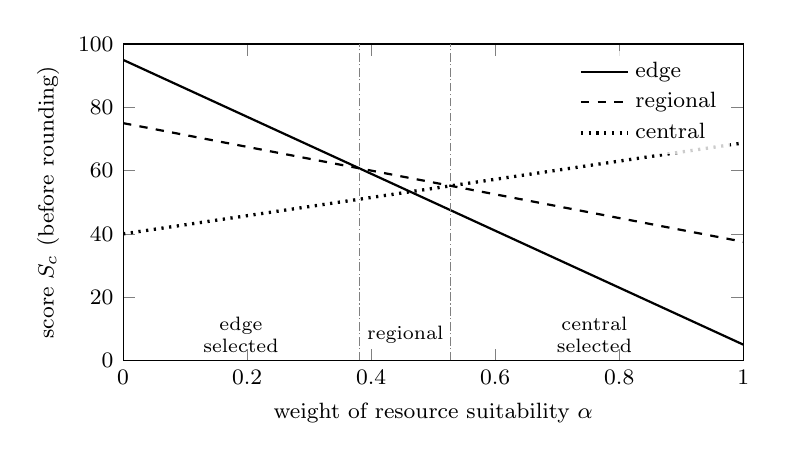
\begin{tikzpicture}
\begin{axis}[
  width=0.78\textwidth, height=5.6cm,
  xmin=0, xmax=1, ymin=0, ymax=100,
  xlabel={weight of resource suitability $\alpha$}, ylabel={score $S_c$ (before rounding)},
  xtick={0,0.2,0.4,0.6,0.8,1}, ytick={0,20,40,60,80,100},
  legend style={at={(0.98,0.98)}, anchor=north east, font=\footnotesize, draw=none, fill=white, fill opacity=0.8, text opacity=1},
  legend cell align=left,
  tick label style={font=\footnotesize}, label style={font=\footnotesize},
  every axis plot/.append style={thick, samples=2, domain=0:1},
]
\addplot[black, solid]        {100*(0.95 - 0.900*x)};  \addlegendentry{edge}
\addplot[black, dashed]       {100*(0.75 - 0.375*x)};  \addlegendentry{regional}
\addplot[black, dotted, very thick] {100*(0.40 + 0.2875*x)}; \addlegendentry{central}
\draw[gray, densely dashdotted] (axis cs:0.381,0) -- (axis cs:0.381,100);
\draw[gray, densely dashdotted] (axis cs:0.528,0) -- (axis cs:0.528,100);
\node[font=\scriptsize, align=center] at (axis cs:0.19,8) {edge\\selected};
\node[font=\scriptsize, align=center] at (axis cs:0.455,8) {regional};
\node[font=\scriptsize, align=center] at (axis cs:0.76,8) {central\\selected};
\end{axis}
\end{tikzpicture}

\caption{Score of each cluster in the scenario of Tab.~\ref*{tab:example} as a function of $\alpha$ (analytic, no measured data)}\label{fig:regions}
\end{figure}

\subsection{Behaviour with missing and stale measurements}\label{sec:analysis-missing}

\Cref{tab:missing} applies the validity rules of \cref{sec:method-validity} to the same scenario. When only the measurement of regional is stale, regional obtains $N = 0$ and is no longer preferred; the stale value neither helps nor removes the cluster. When all measurements are stale, the scheduler behaves exactly like the resource-only configuration. When the optional hard bound H4 is used with $\ell_{\max} = 30$ ms, central becomes ineligible and the remaining clusters are ranked as before.

\begin{table}[t]
\caption{Selection in the scenario of Tab.~\ref*{tab:example} under missing data and a hard bound ($\alpha = 0.5$)}\label{tab:missing}
\centering\small\setstretch{1.0}
\begin{tabularx}{\textwidth}{@{}LCC@{}}
\toprule
\textbf{Condition} & \textbf{Scores (edge, regional, central)} & \textbf{Selected} \\
\midrule
All measurements valid & 50, 56, 54 & regional \\
Measurement of regional stale & 50, 19, 54 & central \\
All measurements stale (fallback) & 5, 38, 69 & central \\
Hard bound $\ell_{\max} = 30$ ms (H4) & 50, 56, ineligible & regional \\
\bottomrule
\end{tabularx}
\end{table}

\subsection{Complexity and overhead}\label{sec:analysis-complexity}

For $|\Cset|$ clusters and $|\Kr|$ resources, the score and normalisation procedures perform $O(|\Cset|\,|\Kr|)$ arithmetic operations and read only the in-memory snapshot. The capacity filter calls each registered estimator once per cluster. With the general estimator this is a local computation; the accurate estimator adds a remote call per decision. Karmada already calls the estimators in its selection stage, so the filter repeats an existing computation rather than adding a new kind of cost. The probe costs one measurement and one annotation update per cluster and period, outside the scheduling path. These are analytical statements; the actual overhead has to be measured (\cref{sec:validation}).

\subsection{Design decisions and trade-offs}\label{sec:analysis-tradeoffs}

The design keeps Karmada's own stages and adds information instead of replacing the decision procedure. Compared with an external optimiser \cite{tabatabaei2025cnf}, it gives up global optimality across several workloads in exchange for a closed-form score that is evaluated in the existing pipeline. Compared with a scheduler that replaces Karmada's cluster selection \cite{bregar2026cosmospan}, it gives up joint selection of cluster and node in exchange for compatibility with Karmada's policies, estimators and default behaviour.

Reusing Karmada's estimators for the capacity condition makes the filter consistent with the selection stage, but it also inherits the estimators' limitations: an optimistic aggregate estimate on clusters with several nodes, or a conservative estimate with coarse resource models. Using the request-based resource summary avoids a dependency on a monitoring system, at the cost of ignoring unrequested load. Treating missing measurements pessimistically prevents an unmeasured cluster from being preferred, but a cluster whose probe fails is disadvantaged even if it is close to the clients; the fallback limits this effect to the case of partial failure. Annotations avoid scheduling churn but are not versioned, so the probe and the scheduler have to agree on the schema. Finally, the single client vantage point keeps the model simple but represents only one client population; several populations would require one measurement per population and a way for a workload to name its population.
